\chapter{一维双曲守恒律方程理论}

\section{预备知识}

物理上有很多的守恒性质,例如能量守恒,质量守恒和动量守恒,这些守恒性质在一定的假设下都可以在数学上对应为如下形式的偏微分方程
\begin{equation}
    \bm{u}_t + \nabla \cdot \bm{F}(\bm{u}) = 0
    \label{eq:cv-laws}
\end{equation}
其中 $x \in \mathbb{R}^d$,满足守恒性质的未知函数 $\bm{u}: \mathbb{R}^d \times \mathbb{R}^+ \to \mathbb{R}^n$,
以及已知的流通量函数 $\bm{F}:\mathbb{R}^m \to \mathbb{R}^n$。

之所以称为守恒律方程,是因为在一个有限的时空区域 $\Omega \times [t^0,t^1] \subset \mathbb{R}^d \times  \mathbb{R}^+$ 对方程~\eqref{eq:cv-laws} 积分可以得到
\[
    0 = \int_{t^0}^{t^1} \int_{\Omega} \left(\bm{u}_t + \nabla \cdot \bm{F}(\bm{u})\right) \,dx\,dt
    = \int_{\Omega} \bm{u}(x,t^1)\,dx - \int_{\Omega} \bm{u}(x,t^0)\,dx
    + \int_{t^0}^{t^1} \int_{\partial \Omega} \bm{n} \cdot \bm{F}(\bm{u}) \,ds\,dt
\]
其中 $\bm{n}$ 是边界处的单位外法向量,最终得到的结果就体现了守恒性质:
\[
    \int_{\Omega} \bm{u}(x,t^1)\,dx - \int_{\Omega} \bm{u}(x,t^0)\,dx
    = - \int_{t^0}^{t^1}\int_{\partial \Omega} \bm{n} \cdot \bm{F}(\bm{u}) \,ds\,dt
\]
$\int_{\Omega} \bm{u}\,dx$ 的变化量仅仅与边界处的交换 $\bm{n} \cdot \bm{F}(\bm{u})$ 有关,
如果 $\bm{n} \cdot \bm{F}(\bm{u})$ 在 $\partial \Omega$ 始终为0,那么就有
\[
    \int_{\Omega} \bm{u}(x,t)\,dx = \text{constant},\,\forall\, t
\]

我们只考虑一维标量情形下的双曲守恒律方程
\begin{equation}
    u_t + f(u)_x = 0,\quad (x,t) \in \mathbb{R} \times  \mathbb{R}^+
    \label{eq:cv-law-scalar}
\end{equation}
考虑纯初值问题或者具有周期边界条件的初边值问题,其中未知函数 $u: \mathbb{R} \times  \mathbb{R}^+ \to \mathbb{R}$,
以及已知的(连续可微的)流通量函数 $f:\mathbb{R} \to \mathbb{R}$。

\begin{example}
    \noindent
    \begin{itemize}
        \item 取 $f(u) = a u$,其中 $a \in \mathbb{R}$ 为常数,就可以得到最简单的常系数线性对流方程
              \[
                  u_t + a u_x = 0
              \]
        \item 取 $f(u) = \frac12 u^2$,就可以得到最简单的非线性守恒律方程——Burgers 方程
              \[
                  u_t + \left(\frac{u^2}2\right)_x = 0
              \]
    \end{itemize}
\end{example}

对于双曲守恒律方程,如果 $f(u)$ 具有足够光滑性,不妨记 $f'(u) = a(u)$,得到两种形式
\begin{enumerate}
    \item 守恒形式 $u_t + f(u)_x = 0$
    \item 非守恒形式 $u_t + a(u) u_x = 0$
\end{enumerate}
从这两种形式出发设计的差分格式并不等价,具有不同的性质和求解效果。

对于双曲守恒律方程,有一类特殊的问题称为 Riemann 问题:
\[
    \left\{
    \begin{aligned}
        u_t + f(u)_x & = 0,\quad (x,t) \in \mathbb{R} \times  \mathbb{R}^+ \\
        u(x,0)       & =
        \begin{cases}
            u_L & x < 0 \\
            u_R & x > 0
        \end{cases}
    \end{aligned}
    \right.
\]
即 $u(x,t)$ 在 $x = 0$ 的左右两侧分别有不同的常数初值 $u_L \neq u_R$。
对于 Riemann 问题,$f(u)$ 的性质以及 $u_L$ 和 $u_R$ 的取值不同会对解的形态产生显著影响。
在下文中对 Riemann 问题的分类讨论中,我们通常会忽略 $u_L = u_R$ 的平凡情况。

\section{特征线}

双曲型方程具有特征线的性质,例如
\begin{itemize}
    \item \textbf{常系数线性对流方程:} $u_t + a u_x = 0$,从 $x=x_0$ 发出的特征线 $x=x(t)$ 满足如下方程
          \[
              \left\{
              \begin{aligned}
                  \frac{d x(t)}{d t} & = a,   \\
                  x(0)               & = x_0.
              \end{aligned}
              \right. \quad \Rightarrow \quad x = x_0 + a t
          \]
          特征线为 $t\!-\!x$ 平面的一族平行直线,斜率由$a$确定。由于
          \[
              \frac{d}{d t}u(x(t),t) = u_x \frac{d x}{d t} + u_t = a u_x + u_t = 0
          \]
          因此解 $u = u(x(t),t)$ 的值沿着特征线不变。
    \item \textbf{变系数线性对流方程:} $u_t + a(x,t) u_x = 0$,其中 $a(x,t)$ 为已知的连续函数,从 $x=x_0$ 发出的特征线 $x=x(t)$ 满足如下方程
          \[
              \left\{
              \begin{aligned}
                  \frac{d x(t)}{d t} & = a(x(t),t), \\
                  x(0)               & = x_0.
              \end{aligned}
              \right.
          \]
          特征线为 $t\!-\!x$ 平面的一族互不相交的曲线。由于
          \[
              \frac{d}{d t}u(x(t),t) = u_x \frac{d x}{d t} + u_t = a(x,t) u_x + u_t = 0
          \]
          因此解 $u = u(x(t),t)$ 的值沿着特征线不变。
    \item \textbf{双曲守恒律方程:} $u_t + f(u)_x = 0$,从 $x=x_0$ 发出的特征线 $x=x(t)$ 满足如下方程
          \[
              \left\{
              \begin{aligned}
                  \frac{d x(t)}{d t} & = f'(u(x(t),t)), \\
                  x(0)               & = x_0.
              \end{aligned}
              \right.
          \]
          由于
          \[
              \frac{d}{d t}u(x(t),t) = u_x \frac{d x}{d t} + u_t = f'(u) u_x + u_t = 0
          \]
          因此解 $u = u(x(t),t)$ 的值沿着特征线不变,进而得到特征线的斜率不变
          \[
              \frac{d x(t)}{d t} = f'(u(x(t),t)) = f'(u(x_0,0))
          \]
          特征线为 $t\!-\!x$ 平面的一族可能相交的直线,斜率由初值确定
          \[
              x(t) = x_0 + f'(u(x_0,0)) t
          \]
\end{itemize}
特征线的性质可以被用来进行精确求解,或者用于设计数值格式等。


\begin{example}
    Burgers方程 $u_t + \left(\frac{u^2}2\right)_x = 0$ 的特征线满足
    \[
        \frac{d x}{d t} = f'(u_0(x_0)) = u_0(x_0)
    \]
    特征线为 $x\!-\!t$ 平面的直线,斜率由特征线经过的初值点决定
    \[
        x = x_0 + u_0(x_0) t
    \]
    因此,如果希望得到精确解 $u(x,t)$,假设存在唯一的 $x_0$ 满足上式,由于沿着特征线值不变,
    便有 $u(x,t) = u_0(x_0)$。
    由于上式为非线性方程,可以通过牛顿迭代法求解
    \[
        x_0^{(k+1)} = x_0^{(k)} - \frac{x_0^{(k)}-x+u_0(x_0^{(k)})t}{1 + u_0'(x_0^{(k)})t}
    \]
    如果牛顿迭代法收敛,那么就有 $x_0^{(k)} \to x_0$ .
\end{example}

双曲守恒律的特征线的斜率由初值确定,特征线可能在某些位置出现相交或者发散,这导致解随着时间演化会产生各种复杂的结构,有如下结论:

\begin{theorem}
    对于严格凸的 $f$,假设给定光滑的初值 $u_0(x)$,满足 $\min f''(u_0(x)) u_0'(x) < 0$,
    那么守恒律方程 $u_t + f(u)_0 = 0$ 的解在短时间内可以保持光滑,
    但是在临界时刻会出现特征线相交,在特征线相交位置会产生无穷斜率(接触间断,激波),经典解不再存在。
    临界时刻 $T_b$ 为
    \[
        T_b = \frac{-1}{\min_x f''(u_0(x)) u_0'(x)}
    \]
\end{theorem}

\begin{proof}
    首先证明在 $T_b$ 时刻特征线首次相交:
    从 $(\xi,0)$ 发出的特征线记作 $l_\xi: x = \xi + f'(u_0(\xi))t$,
    定义集合 $\Omega$
    \[
        \Omega = \{(\xi,\eta) \,|\,  (\xi-\eta)(f'(u_0(\xi)) - f'(u_0(\eta))) < 0\}
    \]
    由于存在某些点满足 $f''(u_0(x)) u_0'(x)<0$,可以保证集合 $\Omega$ 非空。
    在集合 $\Omega$ 上定义二元函数 $T(\xi,\eta)$ 为直线 $l_\xi$ 和 $l_\eta$ 的相交时刻,并对相交时刻取极小值
    \begin{align*}
         & x = \xi + f'(u_0(\xi)) T(\xi,\eta) = \eta + f'(u_0(\eta))T(\xi,\eta)                                                                       \\
         & T(\xi,\eta) = \frac{-1}{\left(\frac{f'(u_0(\xi))-f'(u_0(\eta))}{\xi-\eta}\right)} > 0 ,\quad \forall\, (\xi,\eta) \in \Omega               \\
         & \inf_{(\xi,\eta)\in \Omega} T(\xi,\eta) = \frac{-1}{\inf_{(\xi,\eta)\in \Omega} \left(\frac{f'(u_0(\xi))-f'(u_0(\eta))}{\xi-\eta}\right) }
        = \frac{-1}{\min_x f''(u_0(x)) u_0'(x)} =: T_b
    \end{align*}
    然后证明在 $T_b$ 时刻会出现无穷斜率:设 $(x,t)$ 位于从 $(\xi,0)$ 发出的特征线 $l_\xi$ 上,那么
    \[
        \left\{
        \begin{aligned}
             & x = \xi + f'(u_0(\xi))\, t \\
             & u(x,t) = u_0(\xi)
        \end{aligned}
        \right.
    \]
    在短时间内没有特征线相交,此时 $\xi = \xi(x,t)$ 可以由 $(x,t)$ 隐式确定。对上式关于 $x$ 求导得到
    \begin{align*}
         & 1 = \frac{\partial \xi}{\partial x} + f''(u_0(\xi)) u_0'(\xi) \frac{\partial \xi}{\partial x} \,t \\
         & \frac{\partial u(x,t)}{\partial x} = u_0'(\xi)\frac{\partial \xi}{\partial x}
    \end{align*}
    消去 $\frac{\partial \xi}{\partial x}$ 得到解 $u(x,t)$ 在 $t$ 时刻在 $x$ 处的斜率
    \begin{align*}
        \frac{\partial u(x,t)}{\partial x} =
        \frac{u_0'(\xi)}{1+f''(u_0(\xi)) u_0'(\xi)\,t}
    \end{align*}
    假设 $x_*=\text{argmin}_x f''(u_0(x))u_0'(x)$,那么在 $t \to T_b^-$ 时,在 $x_*$ 处的斜率便会趋于无穷,解产生间断,并且间断出现的位置与特征线首次相交的位置一致
    \[
        \left|\frac{\partial u(x,t)}{\partial x}\right| =  \left|\frac{u_0'(\xi)}{1+f''(u_0(\xi)) u_0'(\xi)\,t}\right| \to \infty,
        \quad \text{as}\,\,\, t \to T_b^-  \qedhere
    \]
\end{proof}

考虑光滑初值 $u_0(x) = \sin(x)$ 的 Burgers 方程,由特征线分布可知,解在形态上会从 $x=\pi$ 的两侧向中间汇聚,随着时间演化,在 $t \ge T_b = 1$ 之后会在 $x=\pi$ 位置出现间断,如图~\ref{fig:burgers-sin}。
在 $t > T_b$ 时不存在满足守恒律方程微分形式的经典解。

\begin{figure}[htbp]
    \centering
    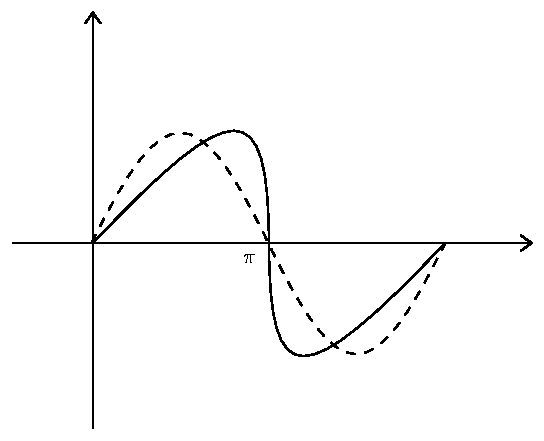
\includegraphics[width=0.4\textwidth]{tikz/burgers-sin.pdf}
    \caption{Burgers方程使用初值 $u_0(x) = \sin(x)$,随着时间演化,解会在 $x=\pi$ 位置出现间断} \label{fig:burgers-sin}
\end{figure}

\section{弱解}

对于双曲守恒律方程,即使初值足够光滑,解也可能随着时间演化产生间断等复杂结构,在间断位置显然不连续、不可导,不可能满足守恒律方程微分形式,
此时无法找到满足要求的解(经典解,古典解),或者说在经典解的范围内解不存在,需要扩大解的范围。

\begin{definition}[弱解定义之一]
    称函数 $u(x,t) \in L^\infty(\mathbb{R}\times(0,+\infty);\mathbb{R})$ 为双曲守恒律方程~\eqref{eq:cv-law-scalar} 的弱解,如果对于任意函数 $\varphi(x,t) \in C_0^\infty(\mathbb{R} \times \mathbb{R}^+)$,都有下式成立
    \[
        \int_{0}^{+\infty} \int_{\mathbb{R}} (u \varphi_t + f(u)\varphi_x)\,dx\,dt
        + \int_{\mathbb{R}} u(x,0)\varphi(x,0)\,dx = 0
    \]
\end{definition}

\begin{definition}[弱解定义之二]
    称函数 $u(x,t) \in L^\infty(\mathbb{R}\times(0,+\infty);\mathbb{R})$ 为双曲守恒律方程~\eqref{eq:cv-law-scalar} 的弱解,如果对于任意有界区域 $[x_L,x_R] \times [t^0,t^1] \subset \mathbb{R} \times \mathbb{R}^+$,都有下式成立
    \[
        \int_{x_L}^{x_R} u(x,t^1)\,dx - \int_{x_L}^{x_R} u(x,t^0)\,dx
        = \int_{t^0}^{t^1} f(u(x_L,t))\,dt - \int_{t^0}^{t^1} f(u(x_R,t))\,dt
    \]
\end{definition}

\begin{remark}
    可以证明对于弱解的两种定义是等价的。
    由于弱解的定义中只涉及到积分,在零测集上的修改不会产生影响,如果两个弱解仅在零测集上不同,那么我们将其视作同一个弱解。在下文表述中的逐点成立应当视作几乎处处成立。
\end{remark}

弱解是比经典解更大的概念,因为弱解对于函数的光滑性没有要求。
如果方程有一个经典解 $u \in C_0^1(\mathbb{R}\times(0,+\infty);\mathbb{R})$,那么使用分部积分就可以证明它也是弱解。

\begin{example}
    取 $f(u) = a u$,其中 $a$ 为常数。对于方程 $u_t + a u_x = 0$ 和任意初值 $u_0(x)$,
    只有在 $u_0(x)$ 具有足够光滑性时,函数 $u(x,t) = u_0(x - a t)$ 才是原方程的经典解。
    但是只要 $u_0(x)$ 具有可积性,函数 $u(x,t) = u_0(x - a t)$ 始终是原方程的弱解。
\end{example}



下面关注由分片经典解组成的函数,它可能在拼接位置没有足够的光滑性,从而不是经典解,
但是只需要在分界面上满足体现局部守恒性的Rankine-Hugoniot条件,就仍然是满足定义的弱解。

\begin{theorem}[分片弱解的刻画,Rankine-Hugoniot jump condition]\label{thm:rh-jump}
    考虑一个时空区域 $\Omega \subset \mathbb{R} \times (0,+\infty)$,假设 $\Omega$ 被一个光滑的时空曲线 $\Gamma$ 划分为两个部分:$\Omega_1,\Omega_2$,
    假设 $u_l(x,t),u_r(x,t)$ 分别是守恒律方程 $u_t + f(u)_x = 0$ 在区域 $\Omega_1,\Omega_2$ 的经典解,
    考虑定义在整个区域 $\Omega$ 上的函数
    \[
        u(x,t) =
        \left\{
        \begin{aligned}
             & u_l(x,t), & (x,t) \in \Omega_1 \\
             & u_r(x,t), & (x,t) \in \Omega_2
        \end{aligned}
        \right.
    \]
    那么 $u$ 是弱解等价于:在时空曲线 $\Gamma$ 上逐点成立
    \[
        \left[f(u_r(x)) - f(u_l(x))\right]n_x +
        \left[u_r(x) - u_l(x)\right]n_t = 0, \quad \forall\, (x,t) \in \Gamma \cap \Omega
    \]
    其中 $\bm{n}=(n_x,n_t)$ 是曲线 $\Gamma$ 在 $x$ 处的单位法向量。
\end{theorem}

\begin{proof}
    任取测试函数 $\varphi(x,t) \in C_0^\infty(\mathbb{R} \times \mathbb{R}^+;\mathbb{R})$,
    由于 $u$ 在 $\Omega_i$ 内部是连续可微的经典解,逐点成立 $u_t + f(u)_x = 0$,可以使用分部积分得到下式
    \[
        \int_{\Omega_i}[u \varphi_t + f(u) \varphi_x]\,dx\,dt
            ={}  - \int_{\Omega_i}
        [u_t \varphi + f(u)_x \varphi]\,dx\,dt
        + \int_{\partial \Omega_i}
        [ n_x f(u) + n_t u] \varphi\,ds
    \]
    对于整个区域 $\Omega$ 有
    \begin{align*}
            & \int_{\Omega}[u \cdot \varphi_t + f(u) \cdot \varphi_x]\,dx\,dt
        \\
        ={} & \sum_{i=1}^2 \left\{
        - \int_{\Omega_i}
        [u_t \cdot \varphi + f(u)_x \cdot \varphi]\,dx\,dt
        + \int_{\partial \Omega_i}
        [ n_x f(u) + n_t u]\cdot \varphi\,ds
        \right\}
        \\
        ={} & 0  - \int_{\mathbb{R}} u(x,0)\varphi(x,0)\,dx + \int_{\Gamma}[ n_x f(u_l) + n_t u_l]\cdot \varphi\,ds
        - \int_{\Gamma}[ n_x f(u_r) + n_t u_r]\cdot \varphi\,ds
    \end{align*}
    这里 $- \int_{\mathbb{R}} u(x,0)\varphi(x,0)\,dx$ 是在$t\!-\!x$上半平面的下边界(即实轴上)进行的边界积分得到的,
    此时 $n_x f(u) + n_t u = - u$;
    $\bm{n}=(n_x,n_t)$ 是时空曲线 $\Gamma$ 在 $x$ 处的单位法向量(从 $\Omega_1$ 指向 $\Omega_2$)。
    由 $\varphi$ 的任意性可知,$u$ 是弱解等价于在时空曲线 $\Gamma$ 上逐点成立
    \[
        \left[f(u_r(x)) - f(u_l(x))\right]n_x +
        \left[u_r(x) - u_l(x)\right]n_t = 0, \quad \forall\, x \in \Gamma \cap \Omega \qedhere
    \]
\end{proof}

在定理~\ref{thm:rh-jump} 的条件下,考虑一个更具体的情况:一条连续可微的时空曲线 $\Gamma: x=x(t),\, t \ge 0$ 将整个 $x-t$ 上半平面划分为左右两个区域:
\[
    \Omega_1 = \{(x,t) \mid x < x(t), t \ge 0\},
    \Omega_2 = \{(x,t) \mid x > x(t), t \ge 0\}.
\]
这两个时空区域在任意固定时刻的切片就是实轴的两个无界区间 $\Omega_1(t) =(-\infty,x(t))$ 和 $\Omega_2(t) = (x(t),+\infty)$,分界点为 $x=x(t)$。
单位法向量可以取作
\[
    \bm{n} = (n_x,n_t) = \frac{1}{\sqrt{1+(x'(t))^2}} (1,-x'(t))
\]
此时定理~\ref{thm:rh-jump} 中的条件即
\[
    \left[f(u_r(x)) - f(u_l(x))\right] - \left[u_r(x) - u_l(x)\right]x'(t) = 0, \quad \forall\, (x,t) \in \Gamma \cap \Omega
\]
如果记分界点的移动速度为 $s = x'(t)$,就可以得到 R-H 条件最常见的形式
\begin{equation}
    f(u_r) - f(u_l) = s\,(u_r - u_l).\label{eq:rh-jump}
\end{equation}


\begin{example}
    下面是 Burgers 方程的 “N波” 解:
    \[
        u(x,t) =
        \begin{cases}
            x/t, & -\sqrt{t} < x < \sqrt{t} \\
            0,   & \text{otherwise}
        \end{cases}
    \]
    “N波” 解由三片经典解组成,左右各存在一个间断 $x = \pm \sqrt{t}$,
    可以验证均满足 R-H 条件
    \[
        \frac{f(u_r) - f(u_l)}{u_r - u_l} =
        \frac{\frac{1}{2t} - 0}{- \frac{1}{\sqrt{t}} - 0} = -\frac{1}{2\sqrt{t}} = s_-,
        \qquad
        \frac{f(u_r) - f(u_l)}{u_r - u_l} =
        \frac{0 - \frac{1}{2t}}{0 - \frac{1}{\sqrt{t}}} = \frac{1}{2\sqrt{t}} = s_+,
    \]
    因此 “N波” 解是弱解。
\end{example}

\begin{remark*}
    若守恒律方程问题的初值为零,$u(x,t) = 0$ 显然是一个满足要求的弱解,
    但是上例的 “N波” 解也给出了一个弱解,这表明弱解不具有唯一性。
\end{remark*}

一个容易忽视的问题是:对守恒律方程微分形式的“等价变换”并不是真正等价的,考虑在 Burgers 方程的两侧乘以 $2u$ 并整理可得
\[
    (u^2)_t + \left(\frac{2}3 u^3\right)_x = 0, \quad
    \xrightarrow{u^2 = v} \quad
    v_t + \left(\frac{2}3 v^{3/2}\right)_x = 0
\]
这个方程看似和 Burgers 方程等价,但是分别考虑两个方程的 R-H 条件可得
\[
    s_1 = \frac{\frac12 u_r^2 - \frac12 u_l^2}{u_r - u_l}
    \quad \neq \quad
    s_2 = \frac{\frac23 u_r^3 - \frac32 u_l^3}{u_r^2 - u_l^2}
\]
两个方程对应的 R-H 条件不一致,这表明满足两个方程的弱解是不同的。
这种差异出现的原因是:对于方程微分形式的上述变形仅在 $u$ 光滑时是等价的,一旦考虑非光滑的弱解,变形就不再等价。


\begin{example}\label{eg:burgers-riemann-jump}
    对于 Burgers 方程的 Riemann 问题($u_L \neq u_R$)
    \[
        \left\{
        \begin{aligned}
            u_t + \left(\frac{u^2}2\right)_x & = 0,\quad (x,t) \in \mathbb{R} \times  \mathbb{R}^+ \\
            u(x,0)                           & =
            \begin{cases}
                u_L & x < 0 \\
                u_R & x > 0
            \end{cases}
        \end{aligned}
        \right.
    \]
    考虑具有如下形式的解:分界面以固定速度 $s$ 移动,分界面两侧保持常值
    \[
        u(x,t) =
        \begin{cases}
            u_L, & x/t < s \\
            u_R, & x/t > s
        \end{cases}
    \]
    解是弱解等价于分界面的移动速度 $s$ 满足 R-H 条件
    \[
        f(u_R)-f(u_L) = s (u_R - u_L),
        \quad \Rightarrow \quad
        s = \frac{f(u_R)-f(u_L)}{u_R - u_L} = \frac{u_L + u_R}{2}
    \]
    因此下面的分片常数解是弱解
    \[
        u(x,t) =
        \begin{cases}
            u_L, & x/t < s \\
            u_R, & x/t > s
        \end{cases},\quad s = \frac12(u_L + u_R)
    \]
    解和特征线分布如图~\ref{fig:burgers-riemann-jump} 所示。
\end{example}

\begin{figure}[htbp]
    \centering
    \begin{subfigure}[b]{0.47\textwidth}
        \centering
        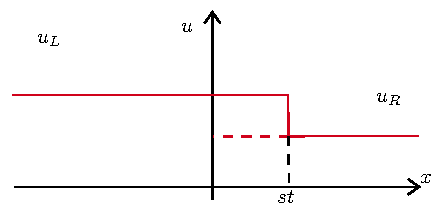
\includegraphics[width=\textwidth]{tikz/burgers-jump-1.pdf}
        \caption{$u_L > u_R$,解的形态}
    \end{subfigure}
    \begin{subfigure}[b]{0.47\textwidth}
        \centering
        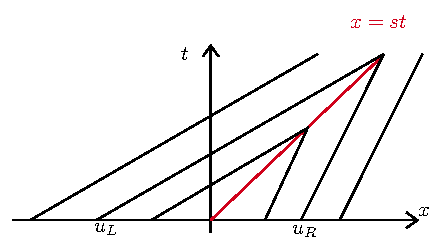
\includegraphics[width=\textwidth]{tikz/burgers-jump-1-lines.pdf}
        \caption{$u_L > u_R$,特征线汇聚}
    \end{subfigure}
    \begin{subfigure}[b]{0.47\textwidth}
        \centering
        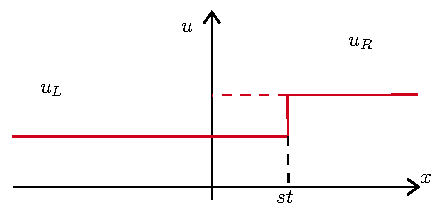
\includegraphics[width=\textwidth]{tikz/burgers-jump-2.pdf}
        \caption{$u_L < u_R$,解的形态}
    \end{subfigure}
    \begin{subfigure}[b]{0.47\textwidth}
        \centering
        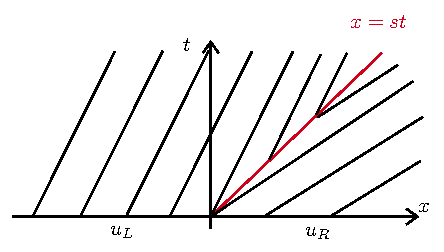
\includegraphics[width=\textwidth]{tikz/burgers-jump-2-lines.pdf}
        \caption{$u_L < u_R$,特征线发散}
    \end{subfigure}
    \caption{Burgers 方程 Riemann 问题的分片常数形式的解及其特征线分布}
    \label{fig:burgers-riemann-jump}
\end{figure}


从经典解到弱解虽然扩大了解的范围,但是弱解却不具有唯一性。
由于问题通常具有实际物理背景,必然存在唯一的解与实际的物理现象对应。
有一些方法可以在弱解范围内进一步筛选出唯一的合理的解,例如熵解和黏性解。

\section{熵解}

\begin{definition}[熵函数和熵通量]
    称函数 $\eta: \mathbb{R} \to \mathbb{R}$ 为熵函数,如果满足:$\eta \in C^2(\mathbb{R})$,并且$\eta'' \ge 0$。
    称函数 $\xi: \mathbb{R} \to \mathbb{R}$ 为对应的熵通量,如果满足 $\xi'(u) = \eta'(u) f'(u)$。
    称熵函数和对应的熵通量组成的二元组 $(\eta,\xi)$ 为一个熵对。
\end{definition}

\begin{example}
    考虑Burgers方程,例如取熵函数 $\eta(u) = \frac{1}{2} u^2$ 和熵通量 $\xi(u) = \frac{1}{3} u^3$,就满足熵对的所有要求。
    再例如取熵函数
    \[
        \eta(u) = \frac{1}{2p} u^{2p} + \frac{\alpha}2 u^2,\quad (p \in \mathbb{N}, p \ge2, \alpha > 0)
    \]
    计算可得 $\eta''(u) = (2p-1) u^{2p-2} + \alpha > 0$,代入计算可得
    \[
        \xi(u) = \frac{1}{2p+1} u^{2p+1} + \frac{\alpha}3 u^3
    \]
    任取参数 $p,\alpha$ 即可构造一组熵对 $(\eta,\xi)$ 。
\end{example}

\begin{definition}
    称方程 $u_t + f(u)_x = 0$ 的弱解 $u(x,t)$ 是熵解,如果满足:对于所有的熵对 $(\eta,\xi)$,都有如下不等式在弱形式下成立
    \[
        \eta(u)_t + \xi(u)_x \le 0.
    \]
    更具体来说,对于所有的非负测试函数 $\varphi(x,t) \in C_0^\infty(\mathbb{R} \times \mathbb{R}^+;\mathbb{R}^+)$,下式成立
    \[
        - \int_0^{+\infty} \int_{\mathbb{R}}(\eta(u) \varphi_t + \xi(u) \varphi_x) \,dx\,dt
        - \int_{\mathbb{R}} \eta(u(x,0))\varphi(x,0)\,dx \le 0
    \]
\end{definition}


显然根据定义可知,熵解一定是弱解,还需要说明的是:经典解(如果存在)一定是熵解。
假设方程有经典解 $u(x,t)$,那么直接对方程乘以 $\eta'(u)$ 可以得到
\begin{gather*}
    \eta'(u) u_t + \eta(u)' f'(u) u_x = 0 \\
    \eta(u)_t + \xi(u)_x = 0
\end{gather*}
因此也满足不等式条件。
这其实也表明熵解在足够光滑的区域可以保持等号成立,在不够光滑的区域可能导致小于号严格成立。

和弱解类似,熵解的定义不易验证,我们仍然关注由分片经典解组成的函数:它是弱解当且仅当在分界面上满足 R-H 条件;它是熵解也等价于在分界面上满足一定的条件。

\begin{theorem}[分片熵解的刻画]
    考虑定义在区域 $\Omega$ 上的由分片经典解组成的函数
    \[
        u(x,t) =
        \left\{
        \begin{aligned}
             & u_l(x,t), & (x,t) \in \Omega_1 = \{(x,t) \mid x < x(t), t \ge 0\} \\
             & u_r(x,t), & (x,t) \in \Omega_2 = \{(x,t) \mid x > x(t), t \ge 0\}
        \end{aligned}
        \right.
    \]
    其中$\Gamma: x=x(t)$ 是一条连续可微的时空曲线,$u_l(x,t)$和$u_r(x,t)$ 分别是区域 $\Omega_1,\Omega_2$ 中的经典解。
    如果 $u(x,t)$ 和分界面移动速度 $s = x'(t)$ 满足 R-H 条件~\eqref{eq:rh-jump},
    那么 $u$ 是熵解等价于:对于任意熵对 $(\eta,\xi)$,在时空曲线 $\Gamma$ 上逐点成立
    \begin{equation} \label{eq:entropy-jump}
        \left[\xi(u_r) - \xi(u_l)\right] - \left[\eta(u_r) - \eta(u_l)\right] x'(t) \le 0, \quad \forall\, (x,t) \in \Gamma \cap \Omega
    \end{equation}
\end{theorem}

\begin{proof}
    与 R-H 条件的证明过程类似。
\end{proof}

\begin{example}
    验证例~\ref{eg:burgers-riemann-jump} 提供的弱解是否是熵解。
    例如取熵对 $(\eta,\xi) = (u^2, \frac23 u^3)$,代入验证
    \begin{align*}
            & \left[\xi(u_R) - \xi(u_L)\right] - \left[\eta(u_R) - \eta(u_L)\right] x'(t)               \\
        ={} & \left(\frac23 u_R^3 - \frac23 u_L^3\right) - \left(u_R^2 - u_L^2\right) \frac{u_L + u_R}2 \\
        ={} & - \frac16 (u_L - u_R)^3
    \end{align*}
    这表明:例~\ref{eg:burgers-riemann-jump} 在 $u_L < u_R$ 时的弱解不是熵解。
    由于我们无法取遍熵对 $(\eta,\xi)$,目前仍然无法验证在 $u_L > u_R$ 时的解是熵解。
\end{example}

综上所述,经典解、熵解和弱解是三个逐渐扩大的概念,关系如图~\ref{fig:entropy-solution}。
它们之间具有严格包含的关系,即:存在不是经典解的熵解,存在不是熵解的弱解(见下文的说明)。
虽然经典解不能保证存在性,弱解不能保证唯一性,但是介于它们中间的熵解却具有存在唯一性。

\begin{theorem}
    标量双曲守恒律方程的熵解存在且唯一。
\end{theorem}

\begin{figure}[htbp]
    \centering
    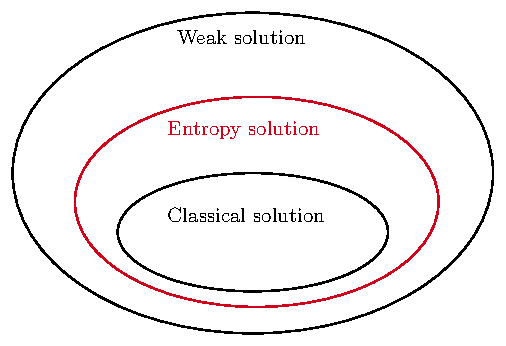
\includegraphics[width=0.5\textwidth]{tikz/entropy-solution.pdf}
    \caption{经典解、熵解和弱解的关系} \label{fig:entropy-solution}
\end{figure}

\section{黏性解}

考虑在原始的方程中加上黏性项,我们关注黏性消失后得到的极限情况,这种做法契合守恒律问题的实际物理背景。

\begin{definition}
    记 $u^{(\varepsilon)}(x,t)$ 为如下方程的解
    \begin{equation}
        u^{(\varepsilon)}_t + f(u^{(\varepsilon)})_x = \varepsilon u^{(\varepsilon)}_{xx},\quad(\varepsilon > 0) \label{eq:limit-solution}
    \end{equation}
    如果存在极限函数
    \[
        u(x,t) := \lim_{\varepsilon \to 0^+} u^{(\varepsilon)}(x,t)
    \]就称其为双曲守恒律方程的黏性解。
\end{definition}

加黏性得到的解通常具有很好的光滑性,但是随着黏性的消失,仍然可以使其收敛到存在间断的弱解。
可以证明:黏性解就是熵解。

\begin{theorem}
    对于满足~\eqref{eq:limit-solution} 的解 $u^{(\varepsilon)}(x,t)$,如果存在极限函数作为黏性解
    \[
        u(x,t) := \lim_{\varepsilon \to 0^+} u^{(\varepsilon)}(x,t)
    \]
    那么黏性解 $u(x,t)$ 就是熵解。
\end{theorem}

\begin{proof}
    $u^{(\varepsilon)}(x,t)$ 满足如下方程
    \[
        u^{(\varepsilon)}_t + f(u^{(\varepsilon)})_x = \varepsilon u^{(\varepsilon)}_{xx}
    \]
    任取熵对 $(\eta,\xi)$,在等式两侧乘以 $\eta'(u^{(\varepsilon)})$ 可得
    \begin{gather*}
        \eta'(u^{(\varepsilon)}) u^{(\varepsilon)}_t + \eta'(u^{(\varepsilon)})f(u^{(\varepsilon)})_x = \varepsilon \eta'(u^{(\varepsilon)}) u^{(\varepsilon)}_{xx}  \\
        \eta_t(u^{(\varepsilon)}) + \eta_x(u^{(\varepsilon)}) =
        \varepsilon \eta_{xx}(u^{(\varepsilon)})
        - \varepsilon \eta''(u^{(\varepsilon)})(u^{(\varepsilon)}_{x})^2
        \le \varepsilon \eta_{xx}(u^{(\varepsilon)})
    \end{gather*}
    取任意的非负测试函数 $\varphi(x,t) \in C_0^\infty(\mathbb{R} \times \mathbb{R}^+;\mathbb{R}^+)$,分部积分可得
    \[
        - \int_0^{+\infty} \int_{\mathbb{R}}(\eta(u^{(\varepsilon)}) \varphi_t + \xi(u^{(\varepsilon)}) \varphi_x) \,dx\,dt
        - \int_{\mathbb{R}} \eta(u^{(\varepsilon)}(x,0))\varphi(x,0)\,dx \le \varepsilon \int_0^{+\infty} \int_{\mathbb{R}}
        \eta(u^{(\varepsilon)}) \varphi_{xx}\,dx\,dt
    \]
    可以证明在 $\varepsilon \to 0^+$ 时,上述不等式的每一项分别收敛到下式的对应项
    \[
        - \int_0^{+\infty} \int_{\mathbb{R}}(\eta(u) \varphi_t + \xi(u) \varphi_x) \,dx\,dt
        - \int_{\mathbb{R}} \eta(u(x,0))\varphi(x,0)\,dx \le 0
    \]
    因此 $u(x,t)$ 是熵解。
\end{proof}


\section{熵条件}

由于前文中对于分片熵解的刻画条件涉及到任意的熵对,不易用于判定,我们需要更实用的熵条件。
考虑分片经典解在分界面处的间断,使用三元组 $(u_l,u_r,s)$ 表示,引入如下定义:

\begin{definition}
    称三元组 $(u_l,u_r,s)$ 为一个熵间断,如果满足 R-H 条件~\eqref{eq:rh-jump},并且对于任意熵对 $(\eta,\xi)$ 都有
    \[
        \left[\xi(u_r) - \xi(u_l)\right] - \left[\eta(u_r) - \eta(u_l)\right] s \le 0
    \]
\end{definition}

\begin{theorem}[Oleinik]
    三元组 $(u_l,u_r,s)$ 为一个熵间断,当且仅当满足 R-H 条件~\eqref{eq:rh-jump} 和 Oleinik 熵条件
    \[
        \frac{f(u_l)-f(v)}{u_l-v} \ge s \ge \frac{f(u_r)-f(v)}{u_r-v},
        \quad \forall\,v \in [\min(u_l, u_r),\,\max(u_l, u_r)]
    \]
\end{theorem}

\begin{proof}
    固定 $(x,t) \in \Gamma \cap \Omega$,任取熵对 $(\eta,\xi)$,条件~\eqref{eq:entropy-jump} 等价于
    \[
        0 \ge{}  \int_{u_l}^{u_r} \left(\xi'(v) - s\, \eta'(v)\right) \,dv
        = \int_{u_l}^{u_r} \eta'(v) \left(f'(v) - s\right) \,dv
    \]
    使用分部积分可以导出下面两个不等式
    \begin{gather*}
        \int_{u_l}^{u_r} \eta''(v) \big[ f(v) - f(u_r) - s(v - u_r) \big] \,dv \ge 0 \\
        \int_{u_l}^{u_r} \eta''(v) \big[ f(v) - f(u_l) - s(v - u_l) \big] \,dv \ge 0
    \end{gather*}
    代入 $s = \frac{f(u_r)-f(u_l)}{u_r - u_l}$ 可知这两个式子是等价的,但是这里使用两种形式便于分别证明两个不等关系。
    因为熵函数 $\eta$ 的任意性以及始终有 $\eta'' \ge 0$,必然有
    \begin{gather*}
        (u_r - u_l) \big[ f(v) - f(u_r) - s(v - u_r) \big] \ge 0,\quad \forall\,v \in [\min(u_l, u_r),\,\max(u_l, u_r)] \\
        (u_r - u_l) \big[ f(v) - f(u_l) - s(v - u_l) \big] \ge 0,\quad \forall\,v \in [\min(u_l, u_r),\,\max(u_l, u_r)]
    \end{gather*}
    整理可得
    \begin{gather*}
        (u_r - u_l)(u_r - v) \left[ s - \frac{f(u_r)-f(v)}{u_r-v} \right] \ge 0,\quad \forall\,v \in [\min(u_l, u_r),\,\max(u_l, u_r)] \\
        (u_r - u_l)(v - u_l) \left[ \frac{f(u_l)-f(v)}{u_l-v} - s\right] \ge 0,\quad \forall\,v \in [\min(u_l, u_r),\,\max(u_l, u_r)]
    \end{gather*}
    无论 $u_l$ 和 $u_r$ 的大小关系如何,对于 $v \in [\min(u_l, u_r),\,\max(u_l, u_r)]$,始终有
    \[
        (u_r - u_l)(u_r - v) \ge 0, \quad (u_r - u_l)(v - u_l) \ge 0
    \]
    因此得证。
\end{proof}

需要结合函数图像来理解 Oleinik 熵条件:定义 $g(u) = f(u_l) + s(u - u_l) = f(u_r) + s(u - u_r)$,也就是过 $(u_l,f(u_l))$ 和 $(u_r,f(u_r))$ 两点的直线,那么 Oleinik 熵条件可以解释为(如图~\ref{fig:oleinik-condition})

\begin{itemize}
    \item 如果 $u_l < u_r$,要求在 $[u_l,u_r]$ 范围内,曲线 $y=f(u)$ 始终在两点连线 $y=g(u)$ 的上方或重合;
    \item 如果 $u_l > u_r$,要求在 $[u_r,u_l]$ 范围内,曲线 $y=f(u)$ 始终在两点连线 $y=g(u)$ 的下方或重合;
\end{itemize}

\begin{figure}[htbp]
    \centering
    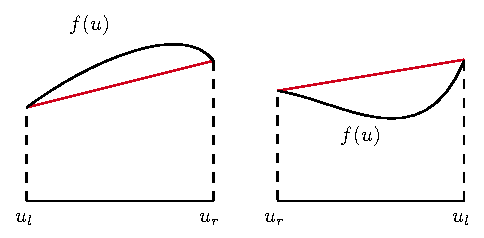
\includegraphics[width=0.6\textwidth]{tikz/oleinik-condition.pdf}
    \caption{Oleinik 熵条件的解释} \label{fig:oleinik-condition}
\end{figure}

对 Oleinik 熵条件中的不等式,直接令 $u \to u_l,u_r$ 可得
\[
    f'(u_l) \ge s \ge f'(u_r)
\]
这个条件被称为 Osher 熵条件。
对于任意可微的 $f(u)$,Osher 熵条件是 Oleinik 熵条件的推论,并不是充要条件,但是如果要求 $f'' \neq 0$,那么两者就是等价的。

由于 $f'(u)$ 的物理意义是物质的移动速度,$s$ 是分界面的移动速度,Osher 熵条件要求:
\begin{itemize}
    \item 左侧物质的移动速度大于等于分界面的移动速度;
    \item 分界面的移动速度大于等于右侧物质的移动速度。
\end{itemize}
由于 $f'(u)$ 在 $x\!-\!t$ 平面上具有明确的几何意义--对应特征线的斜率倒数,Osher 熵条件还可以结合特征线的分布来解释:
\begin{itemize}
    \item 只有间断两侧特征线不断向时空分界面汇聚(或平行),对应的间断解才可能是熵解。
    \item 如果间断两侧特征线呈现发散趋势,那么对应的间断解即使满足局部守恒性,仍然是不合理的。
\end{itemize}


\begin{example}
    对于 Burgers 方程,由于 $f''(u) = 1 >0$ 严格凸,Osher 熵条件是充要的。
    使用 Osher 熵条件检查例~\ref{eg:burgers-riemann-jump} 提供的弱解:
    \begin{gather*}
        f'(u_L) \ge s = \frac{f(u_R)-f(u_L)}{u_R - u_L} \ge f'(u_R), \\
        \Rightarrow \quad u_L \ge s = \frac{u_L + u_R}2 \ge u_R \\
        \Rightarrow \quad u_L \ge u_R
    \end{gather*}
    因此当且仅在 $u_L \ge u_R$ 时,例~\ref{eg:burgers-riemann-jump} 提供的解是熵解。
\end{example}


\section{激波、接触间断和稀疏波}

现在对由分片经典解组成的熵解的形态进行更具体的刻画,其中存在三类典型结构:激波、接触间断和稀疏波,
分别对应着特征线的三种趋势:汇聚,平行,发散。

\begin{definition}
    对于熵间断 $(u_l,u_r,s)$,将其分为两类:
    \begin{itemize}
        \item 称为激波,如果至少存在一个熵对 $(\eta,\xi)$,使得
              \[
                  \left[\xi(u_r) - \xi(u_l)\right] - \left[\eta(u_r) - \eta(u_l)\right] s < 0
              \]
        \item 称为接触间断,如果对于任意熵对 $(\eta,\xi)$,都有
              \[
                  \left[\xi(u_r) - \xi(u_l)\right] - \left[\eta(u_r) - \eta(u_l)\right] s = 0
              \]
    \end{itemize}
\end{definition}

\begin{theorem}
    熵间断 $(u_l,u_r,s)$ 是一个接触间断等价于
    \[
        f(v) = f(u_l) + s(v - u_l) = f(u_r) + s(v - u_r), \quad v \in [\min(u_l, u_r),\,\max(u_l, u_r)]
    \]
    即 $f(u)$ 在这个范围内等于在 $(u_l,f(u_l))$ 和 $(u_r,f(u_r))$ 两点之间的连线。
\end{theorem}

\begin{proof}
    由接触间断的定义可知,$(u_l,u_r,s)$ 和 $(u_r,u_l,s)$ 都是熵间断,即两侧状态交换也不会违背熵条件。
    由 Oleinik 熵条件的图像解释可知,$f(u)$ 既要求在两点之间连线的上方或重合,也要求在两点之间连线的下方或重合,因此 $f(u)$ 必然和两点之间连线完全重合。
\end{proof}

这表明产生接触间断的条件是曲线 $y=f(u)$ 在某一个区间内是直线。
考虑从特征线的角度理解:对于接触间断 $(u_l,u_r,s)$,由于 $f'$ 在 $[\min(u_l, u_r),\,\max(u_l, u_r)]$ 是常值,因此有
\[
    f'(u_l) = s = f'(u_r)
\]
这表明:在 $x\!-\!t$ 平面上,接触间断的两侧特征线平行,并且和时空区域的分界面也平行。从物理角度来说,这表明接触间断的两侧实际并没有发生物质交换,激波的两侧则发生了物质交换。
考虑两个具体的方程:
\begin{itemize}
    \item 对于 Burgers 方程,$f(u) = \frac12 u^2$,由于不存在直线片段,因此产生的熵间断只可能是激波;
    \item 对于线性方程,$f(u) = a u$($a$ 为常数),由于本身就是直线,因此产生的熵间断只可能是接触间断。
\end{itemize}

\begin{example}
    考虑 $f(u) = a u$($a$ 为常数),那么特征线为一组平行的直线。对于初值 $u_0(x) = \chi_{[m,n]}(x)$,由特征线的走向可以直接得到解
    \[
        u(x,t) = u_0(x - a t) = \chi_{[m+at,n+at]}(x)
    \]
    存在两处间断:$(0,1,a)$ 和 $(1,0,a)$,显然均满足 R-H 条件和 Oleinik 熵条件,因此是熵间断,
    根据上述命题可知,这两个熵间断都是接触间断。
\end{example}


重新考虑守恒律方程的微分形式
\[
    u_t + f(u)_x = 0
\]
如果 $f'$ 局部可逆,不妨设 $(f')^{-1}$ 可以定义在区间 $[s^{(l)},s^{(r)}]$,那么可以构造如下形式的(局部)解
\[
    u(x,t) = (f')^{-1}\left(\frac{x-x_0}{t}\right), \quad  x \in [x_0 + s^{(l)}t ,\, x_0 +s^{(r)} t ]
\]
其中 $x_0$ 是任意给定的起点,定义区间是随时间演化逐渐扩大的区间 $[x_0 + s^{(l)}t ,\, x_0 + s^{(r)} t]$,在两端的值记作
\[
    u^{(l)} = (f')^{-1}(s^{(l)}), \quad
    u^{(r)} = (f')^{-1}(s^{(r)})
\]
在 $x\!-\!t$ 平面内,解的所有特征线位于从 $(x_0,0)$ 发出的一个扇形区域
\[
    S = \{(x,t) \mid s^{(l)} t \le x - x_0 \le s^{(r)} t \}
\]
特征线呈现发散趋势,并且特征线斜率从一侧到另一侧连续过渡,如图~\ref{fig:rarefaction}。

\begin{figure}[htbp]
    \centering
    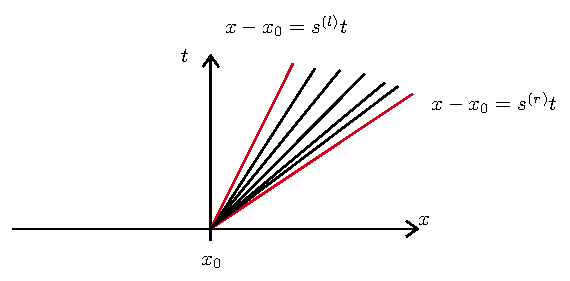
\includegraphics[width=0.6\textwidth]{tikz/rerafaction.pdf}
    \caption{稀疏波对应的特征线分布} \label{fig:rarefaction}
\end{figure}

由构造过程可知,这个局部解具有自相似性,并且在定义区间内是连续的,可以直接验证在区间内部是满足守恒律方程的微分形式
\begin{align*}
    u_t + f(u)_x ={} &
    \frac{1}{f''(u)} (f''(u) u_t + f'(u) f''(u) u_x)                                                                                                 \\
    ={}              & \frac{1}{f''(u)} \left[ \partial_t f'(u) + \partial_x \left( \frac{(f'(u))^2}2 \right)\right]                                 \\
    ={}              & \frac{1}{f''(u)} \left[  \partial_t \left( \frac{x-x_0}{t} \right) + \partial_x \left( \frac{(x-x_0)^2}{2t^2} \right) \right] \\
    ={}              & \frac{1}{f''(u)} \left( - \frac{x-x_0}{t^2} + \frac{x-x_0}{t^2} \right) = 0
\end{align*}

\begin{definition}
    上文构造的(局部)经典解称为(从 $x=x_0$ 发出的)稀疏波。
\end{definition}

\begin{remark*}
    稀疏波解的构造受限于 $f'$ 的局部可逆性,如果 $f'$ 是全局可逆的(例如 $f$ 严格凸),
    那么定义稀疏波解时的参数 $s^{(l)}$ 和 $s^{(r)}$ 可以在 $f'(u)$ 的值域中自由选取。
\end{remark*}

\begin{example}
    考虑 $f(u) = \frac12 u^2$,$f'(u) = u$ 全局可逆,可以构造稀疏波解
    \[
        u(x,t) = (f')^{-1}\left(\frac{x-x_0}{t}\right) = \frac{x-x_0}{t}
    \]
\end{example}

\begin{example}
    考虑 $f(u) = \frac14 u^4$,$f'(u) = u^3$ 全局可逆,可以构造稀疏波解
    \[
        u(x,t) = (f')^{-1}\left(\frac{x-x_0}{t}\right) = \left(\frac{x-x_0}{t}\right)^{\frac13}
    \]
\end{example}

\section{Riemann 问题的熵解}

对于一般的双曲守恒律方程的 Riemann 问题($u_L \neq u_R$)
\[
    \left\{
    \begin{aligned}
        u_t + f(u)_x & = 0,\quad (x,t) \in \mathbb{R} \times  \mathbb{R}^+ \\
        u(x,0)       & =
        \begin{cases}
            u_L & x < 0 \\
            u_R & x > 0
        \end{cases}
    \end{aligned}
    \right.
\]
熵解的显式表达形式过于复杂,但是我们可以给出它的构造。为了描述解的构造过程,我们必须使用一些简化表述,考虑两个状态之间的连接:
\begin{enumerate}
    \item 称左右状态 $u^{(l)}$ 和 $u^{(r)}$ 通过(从$x=0$发出的)稀疏波连接,对应的解为
          \[
              u(x,t) = (f')^{-1}\left(\frac{x}{t}\right), \quad  x \in [f'(u^{(l)}) t ,\, f'(u^{(r)}) t ]
          \]
          这要求 $f'(u^{(l)}) < f'(u^{(r)})$ 以及 $f'$ 在 $[\min(u^{(l)},u^{(r)}),\,\max(u^{(l)},u^{(r)})]$ 是局部可逆的。
          这两个条件也可以表述为:

          \begin{enumerate}
              \item 若 $u^{(l)} < u^{(r)}$,要求 $f'$ 在 $[u^{(l)},u^{(r)}]$ 严格单调增,亦即 $\{ (u,y) \mid y \ge f(u),\, u \in [u^{(l)},u^{(r)}]\}$ 是凸集,并且 $f(u)$ 在这个范围内不是线性的;
              \item 若 $u^{(l)} > u^{(r)}$,要求 $f'$ 在 $[u^{(r)},u^{(l)}]$ 严格单调减,亦即 $\{ (u,y) \mid y \le f(u),\, u \in [u^{(r)},u^{(l)}]\}$ 是凸集,并且 $f(u)$ 在这个范围内不是线性的。
          \end{enumerate}

    \item 称左右状态 $u^{(l)}$ 和 $u^{(r)}$ 通过激波或接触间断连接,对应的解为
          \[
              u(x,t) =
              \begin{cases}
                  u^{(l)}, & x/t < s \\
                  u^{(r)}, & x/t > s
              \end{cases}, \quad s = \frac{f(u^{(r)})-f(u^{(l)})}{u^{(r)} - u^{(l)}}
          \]
          分界面位置为 $x = x(t) = s\,t$,需要满足 Oleinik 熵条件
          \[
              \frac{f(u^{(l)})-f(v)}{u^{(l)}-v} \ge s \ge \frac{f(u^{(r)})-f(v)}{u^{(r)}-v},
              \quad \forall\,v \in [\min(u^{(l)}, u^{(r)}),\,\max(u^{(l)}, u^{(r)})]
          \]
          也可以表述为:记连接 $(u^{(l)},f(u^{(l)}))$ 和 $(u^{(r)},f(u^{(r)}))$ 两点的直线为 $g(u) = f(u^{(l)}) + s(u - u^{(l)})$,那么
          \begin{enumerate}
              \item 若 $u^{(l)} < u^{(r)}$,要求 $g(u) \le f(u)$ 在 $[u^{(l)},u^{(r)}]$ 成立,亦即 $\{ (u,y) \mid y \ge g(u),\, u \in [u^{(l)},u^{(r)}]\}$ 是 $\{ (u,y) \mid y \ge f(u),\, u \in [u^{(l)},u^{(r)}]\}$ 的凸包;
              \item 若 $u^{(l)} > u^{(r)}$,要求 $g(u) \ge f(u)$ 在 $[u^{(r)},u^{(l)}]$ 成立,亦即 $\{ (u,y) \mid y \le g(u),\, u \in [u^{(r)},u^{(l)}]\}$ 是 $\{ (u,y) \mid y \le f(u),\, u \in [u^{(r)},u^{(l)}]\}$ 的凸包。
          \end{enumerate}
\end{enumerate}
然后考虑三个点之间的状态连接:对于左状态 $u^{(l)}$,中状态 $u^{(m)}$ 和右状态 $u^{(r)}$:
\begin{enumerate}
    \item 如果均使用激波或接触间断相连,那么在考虑满足两个状态连接的要求之后,可以推出:左状态可以直接和右状态使用激波或接触间断相连,无需中间状态;
    \item 如果均使用稀疏波相连,那么在考虑满足两个状态连接的要求之后,同样可以推出:左状态可以直接和右状态使用稀疏波相连,无需中间状态;
    \item 如果左状态和中间状态使用激波或接触间断连接,而中间状态到右状态使用稀疏波相连,那么由稀疏波的定义区间和分界面位置可以推出
          \[
              f'(u^{(m)}) = \frac{f(u^{(m)}) - f(u^{(l)})}{u^{(m)} - u^{(l)}}
          \]
          从图像角度来解释,这表明在公共点 $u^{(m)}$,$f(u)$ 的曲线和激波或接触间断对应的直线需要满足相切关系。
    \item 如果左状态和中间状态使用稀疏波连接,而中间状态到右状态使用激波或接触间断相连,同理
          \[
              f'(u^{(m)}) = \frac{f(u^{(r)}) - f(u^{(m)})}{u^{(r)} - u^{(m)}}
          \]
\end{enumerate}

寻找 Riemann 问题的熵解的问题可以转换为:寻找一个单调的状态序列来连接左右初值状态 $u_L$ 和 $u_R$,不妨记作
\begin{align*}
                   & u_L = u^{(1)} < u^{(2)} < \cdots < u^{(k-1)} < u^{(k)} = u_R \\
    \text{or}\quad & u_L = u^{(1)} > u^{(2)} > \cdots > u^{(k-1)} > u^{(k)} = u_R
\end{align*}
如果相邻状态 $u^{(i)}$ 和 $u^{(i+1)}$ 均可以通过激波、接触间断或稀疏波相连,满足前文中讨论的所有条件,
那么就可以得到一个符合要求的熵解,也就是唯一的熵解。

因为我们已经将不同状态之间可以连接的条件全都转换为了图像角度的要求,可以自然诱导出使用凸包来寻找单调状态序列的方法:
对于左右初值 $u_L$ 和 $u_R$ 的 Riemann 问题,引入辅助函数 $g(u)$:
\begin{enumerate}
    \item 若 $u_L < u_R$,定义 $g(u)$,使得$\{ (u,y) \mid y \ge g(u),\, u \in [u_L,u_R]\}$ 是 $\{ (u,y) \mid y \ge f(u),\, u \in [u_L,u_R]\}$ 的凸包;
    \item 若 $u_L > u_R$,定义 $g(u)$,使得$\{ (u,y) \mid y \le g(u),\, u \in [u_L,u_R]\}$ 是 $\{ (u,y) \mid y \le f(u),\, u \in [u_L,u_R]\}$ 的凸包。
\end{enumerate}
由凸包的构造过程可知,$g(u)$ 通常可以使用分段函数表示,不妨记作
\[
    g(u) = g^{(i)}(u), \quad u \in [\min(u^{(i)},u^{(i+1)}),\max(u^{(i)},u^{(i+1)})],\quad i=1,\dots,k-1
\]
并且 $g^{(i)}(u)$ 只有三种互异的情况:
\begin{enumerate}
    \item $g^{(i)}(u) = f(u)$,并且在这个范围内是线性的;
    \item $g^{(i)}(u) = f(u)$,并且在这个范围内不是线性的;
    \item $g^{(i)}(u) \neq f(u)$,而是连接两个端点的直线
          \[
              g^{(i)}(u) = f(u^{(i)}) + s(u - u^{(i)}),\quad s = \frac{f(u^{(i+1)})-f(u^{(i)})}{u^{(i+1)} - u^{(i)}}
          \]
          此时两端点如果不是边界点 $u_L,u_R$,必然满足相切关系 $s = f'(u^{(i)})$,$s = f'(u^{(i+1)})$。
\end{enumerate}
容易验证,通过 $g(u)$ 的分段函数表示自然得到的单调状态序列 $\{u^{(i)}\}$ 满足所有要求。
因此,我们可以给出一般情况下的熵解构造。
\begin{theorem}
    对于一般的 $f$,Rimann 问题的熵解可以通过如下方式构造:
    基于 $u_L$ 与 $u_R$ 的大小关系构造 $f(u)$ 相关的凸包函数 $g(u)$,由 $g(u)$ 的分段表示诱导产生一组状态
    \begin{align*}
                       & u_L = u^{(1)} < u^{(2)} < \cdots < u^{(k-1)} < u^{(k)} = u_R \\
        \text{or}\quad & u_L = u^{(1)} > u^{(2)} > \cdots > u^{(k-1)} > u^{(k)} = u_R
    \end{align*}
    对于相邻状态 $u^{(i)}$ 和 $u^{(i+1)}$:
    \begin{enumerate}
        \item 如果 $g^{(i)}(u) = f(u)$,并且在这个范围内是线性的,那么两个状态应当使用接触间断相连;
        \item 如果 $g^{(i)}(u) = f(u)$,并且在这个范围内不是线性的,那么两个状态应当使用稀疏波相连;
        \item 如果 $g^{(i)}(u) \neq f(u)$,而是连接两个端点的直线,那么两个状态应当使用激波相连。
    \end{enumerate}
    这样得到的解就是 Riemann 问题的熵解。

\end{theorem}

由于一般情况的解的组成比较复杂,难以给出显式的表达形式,但是我们可以考虑一些简单的例子,图~\ref{fig:entropy-solution-general} 展示了几种典型情况,
例如左上图(稀疏波—激波)对应的解为:
\[
    u(x,t) ={}
    \begin{cases}
        u_L,            & x/t < f'(u_L)                       \\
        (f')^{-1}(x/t), & f'(u_L) \le x/t \le f'(u^{(2)}) = s \\
        u_R,            & x/t > f'(u^{(2)}) = s
    \end{cases}
    ,\quad
    s := \frac{f(u_R) - f(u^{(2)})}{u_R - u^{(2)}}
\]
左下图(激波—稀疏波)对应的解的显式表达为:
\[
    u(x,t) ={}
    \begin{cases}
        u_L,            & x/t < f'(u^{(2)}) = s               \\
        (f')^{-1}(x/t), & s = f'(u^{(2)}) \le x/t \le f'(u_R) \\
        u_R,            & x/t > f'(u_R)
    \end{cases}
    ,\quad
    s := \frac{f(u^{(2)}) - f(u_L)}{u^{(2)} - u_L}
\]
图~\ref{fig:entropy-solution-general-2} 给出了一种更复杂的情况:稀疏波—激波—稀疏波,对应的解为:
\[
    u(x,t) ={}
    \begin{cases}
        u_L,            & x/t < f'(u_L)                       \\
        (f')^{-1}(x/t), & f'(u_L) \le x/t < f'(u^{(2)}) = s   \\
        (f')^{-1}(x/t), & s = f'(u^{(3)}) \le x/t \le f'(u_R) \\
        u_R,            & x/t > f'(u_R)
    \end{cases}
    ,\quad
    s := \frac{f(u^{(3)}) - f(u^{(2)})}{u^{(3)} - u^{(2)}}
\]

\begin{figure}[htbp]
    \centering
    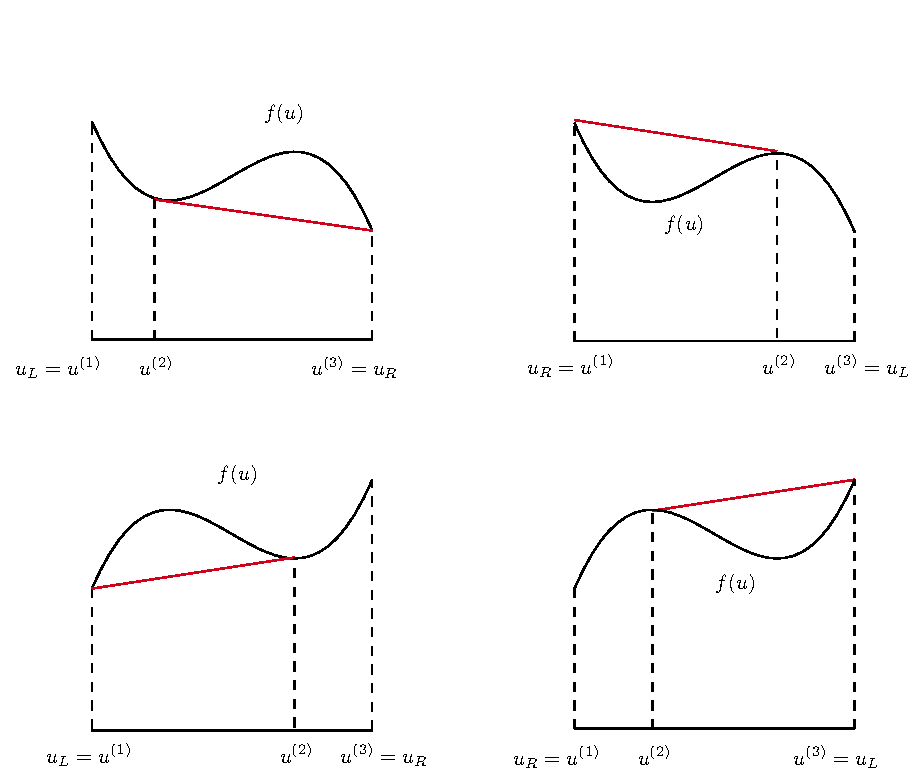
\includegraphics[width=\textwidth]{tikz/entropy-solution-general.pdf}
    \caption{对于一般的 $f$,Riemann 问题的几种熵解结构示意:左上图和右上图代表稀疏波—激波,左下图和右下图代表激波—稀疏波。}
    \label{fig:entropy-solution-general}
\end{figure}

\begin{figure}[htbp]
    \centering
    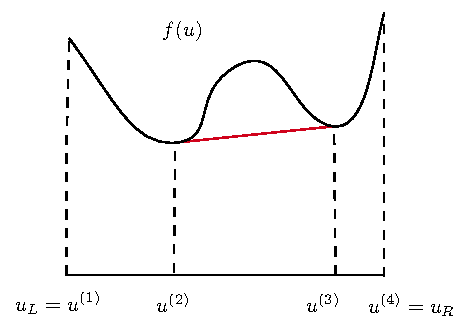
\includegraphics[width=.6\textwidth]{tikz/entropy-solution-general-2.pdf}
    \caption{对于一般的 $f$,Riemann 问题的一种熵解结构示意:稀疏波—激波—稀疏波。}
    \label{fig:entropy-solution-general-2}
\end{figure}


在一般性结论的基础上,考虑 $f'' > 0$ 严格凸的情形,根据上述定理:
\begin{enumerate}
    \item 若 $u_L < u_R$,那么 $g(u) = f(u)$,只存在两个状态 $u_L$ 和 $u_R$,并且必然通过稀疏波相连;
    \item 若 $u_L > u_R$,那么 $g(u) = f(u_L) + s(u - u_L)$ 为两点连线,只存在两个状态 $u_L$ 和 $u_R$,并且必然通过激波相连。
\end{enumerate}
由于此时熵解的构造非常简单,可以直接给出熵解的显式表达。

\begin{theorem}
    对于 $f$ 严格凸的情况,Rimann 问题的熵解为:
    \begin{enumerate}
        \item 如果 $u_L < u_R$,$u(x,t)$ 是一个(从$x=0$发出的)稀疏波,具体为
              \[
                  u(x,t) ={}
                  \begin{cases}
                      u_L,            & x/t < f'(u_L)               \\
                      (f')^{-1}(x/t), & f'(u_L) \le x/t \le f'(u_R) \\
                      u_R,            & x/t > f'(u_R)
                  \end{cases}
              \]
        \item 如果 $u_L > u_R$,$u(x,t)$ 是一个激波,具体为
              \[
                  u(x,t) =
                  \begin{cases}
                      u_L, & x/t < s \\
                      u_R, & x/t > s
                  \end{cases},\quad s = \frac{f(u_R)-f(u_L)}{u_R - u_L}
              \]
    \end{enumerate}
    如图~\ref{fig:entropy-solution-convex} 所示。
\end{theorem}

\begin{figure}[htbp]
    \centering
    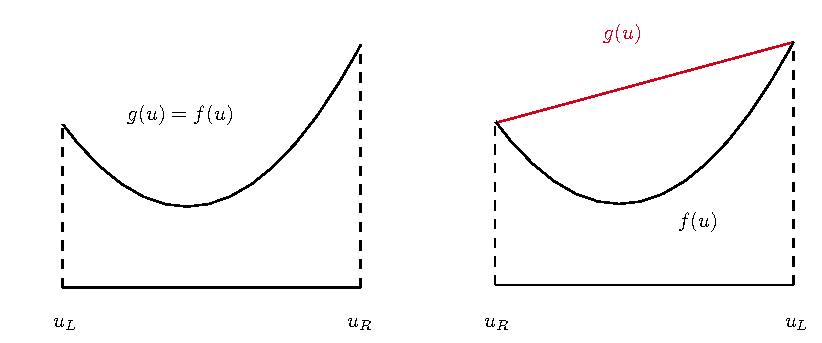
\includegraphics[width=.9\textwidth]{tikz/entropy-solution-convex.pdf}
    \caption{对于严格凸的 $f$,Riemann 问题的熵解结构示意,左图代表稀疏波,右图代表激波。} \label{fig:entropy-solution-convex}
\end{figure}

\begin{example}
    考虑一个典型的 $f$ 非凸非凹的情况—— Buckley-Leverett 方程,对应的 $f(u)$ 具体为
    \[
        f(u) = \frac{u^2}{u^2 + a(1-u)^2}.
    \]
    其中参数 $a > 0$ 给定,通常只关注 $u \in [0,1]$ 的情况。
    我们考虑两个 Riemann 问题:
    \begin{enumerate}
        \item $u_L = 0$,$u_R = 1$;
        \item $u_L = 1$,$u_R = 0$。
    \end{enumerate}
    两种情况下的熵解结构均为稀疏波—激波,具体表达式为
    \[
        u(x,t) ={}
        \begin{cases}
            u_L,            & x/t < f'(u_L)                       \\
            (f')^{-1}(x/t), & f'(u_L) \le x/t \le f'(u^{(2)}) = s \\
            u_R,            & x/t > f'(u^{(2)}) = s
        \end{cases}
        ,\quad
        s := \frac{f(u_R) - f(u^{(2)})}{u_R - u^{(2)}}
    \]
    中间状态 $u^{(2)}$ 的具体值可以通过如下方程解出
    \[
        f'(u^{(2)}) = \frac{f(u_R) - f(u^{(2)})}{u_R - u^{(2)}}
    \]
    熵解结构以及解的形态如图~\ref{fig:buckley-leverett-riemann} 所示。
\end{example}

\begin{figure}[htbp]
    \centering
    \begin{subfigure}[b]{\textwidth}
        \centering
        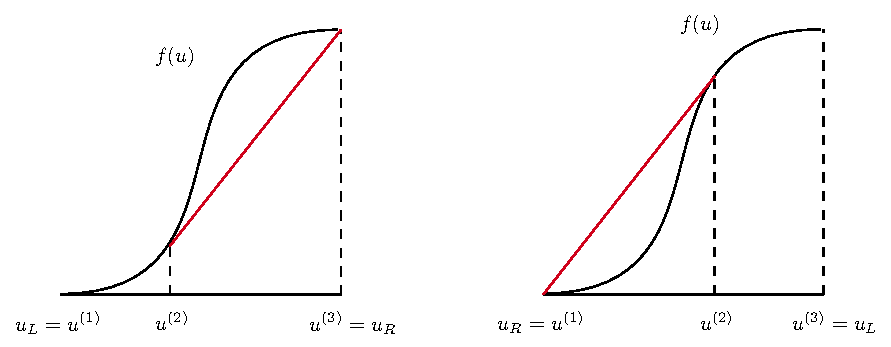
\includegraphics[width=.9\textwidth]{tikz/buckley-leverett-riemann.pdf}
    \end{subfigure}
    \begin{subfigure}[b]{\textwidth}
        \centering
        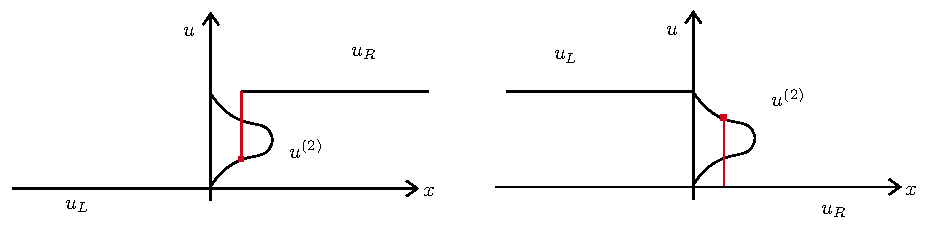
\includegraphics[width=\textwidth]{tikz/buckley-leverett-riemann-plot.pdf}
    \end{subfigure}
    \caption{Buckley-Leverett 方程 Riemann 问题的熵解结构以及解的形态。} \label{fig:buckley-leverett-riemann}
\end{figure}


我们关注 Riemann 问题在分界面 $x=0$ 的解 $u(0,t)$ 以及 $f(u(0,t))$ 的值,需要结合图像进行分类讨论:
\begin{enumerate}
    \item $u_L < u_R$ 时,假设 $f(u)$ 在 $[u_L,u_R]$ 存在唯一的最小值点 $\widetilde{u}_m$,
          它必然也是 $g(u)$ 的最小值点
          \begin{enumerate}
              \item 如果 $\widetilde{u}_m$ 位于某个稀疏波中,那么由于 $f'(\widetilde{u}_m) = 0$,必有 $u(0,t) = \widetilde{u}_m$;
                    否则 $\widetilde{u}_m$ 必然处于激波或接触间断的一端,并且 $\widetilde{u}_m$ 必须为 $u_L$ 或 $u_R$;
              \item 如果 $\widetilde{u}_m = u_L$,这段对应的斜率(间断移动速度)必然大于0,必有 $u(0,t) = u_L = \widetilde{u}_m$;
              \item 如果 $\widetilde{u}_m = u_R$,这段对应的斜率(间断移动速度)必然小于0,必有 $u(0,t) = u_R = \widetilde{u}_m$。
          \end{enumerate}
    \item $u_L > u_R$ 时,假设 $f(u)$ 在 $[u_L,u_R]$ 存在唯一的最大值点 $\widetilde{u}_M$;
          它必然也是 $g(u)$ 的最大值点
          \begin{enumerate}
              \item 如果 $\widetilde{u}_m$ 位于某个稀疏波中,那么由于 $f'(\widetilde{u}_M) = 0$,必有 $u(0,t) = \widetilde{u}_M$;
                    否则 $\widetilde{u}_M$ 必然处于激波或接触间断的一端,并且 $\widetilde{u}_M$ 必须为 $u_L$ 或 $u_R$;
              \item 如果 $\widetilde{u}_M = u_L$,这段对应的斜率(间断移动速度)必然大于0,必有 $u(0,t) = u_L = \widetilde{u}_M$;
              \item 如果 $\widetilde{u}_M = u_R$,这段对应的斜率(间断移动速度)必然小于0,必有 $u(0,t) = u_R = \widetilde{u}_M$。
          \end{enumerate}
\end{enumerate}
整理可得
\[
    u(0,t) =
    \begin{cases}
        \text{argmin}_{[u_L,u_R]} f(u), & u_L < u_R \\
        \text{argmax}_{[u_R,u_L]} f(u), & u_L > u_R
    \end{cases}
\]
如果有多个最值点,那么会在 $x=0$ 位置形成固定不动的激波或接触间断,此时 $u(0,t)$ 无法定义。
但是无论最值点是否唯一,都不影响 $f(u(0,t))$ 的取值
\[
    f(u(0,t)) =
    \begin{cases}
        \text{min}_{[u_L,u_R]} f(u), & u_L < u_R \\
        \text{max}_{[u_R,u_L]} f(u), & u_L > u_R
    \end{cases}
\]
这样就得到了著名的 Godunov flux:
\[
    f^{God}(u_L,u_R) =
    \begin{cases}
        \text{min}_{[u_L,u_R]} f(u), & u_L \le u_R \\
        \text{max}_{[u_R,u_L]} f(u), & u_L > u_R
    \end{cases}
\]

\section{近似 Riemann 解}

在数值格式中,我们通常希望近似求解 Riemann 问题,做法是直接假设 Riemann 问题具有某种典型的结构,然后联列条件求解。

假定左右状态使用激波相连,那么
\[
    u(0,t) =
    \begin{cases}
        u_L, & s \ge 0 \\
        u_R. & s < 0
    \end{cases},
    \quad
    f(u(0,t)) =
    \begin{cases}
        f(u_L), & s \ge 0 \\
        f(u_R). & s < 0
    \end{cases},
    \quad
    s = \frac{f(u_R)-f(u_L)}{u_R - u_L}
\]
这样就得到了 Roe flux:
\[
    f^{Roe}(u_L,u_R) =
    \begin{cases}
        f(u_L), & s \ge 0 \\
        f(u_R). & s < 0
    \end{cases},
    \quad
    s = \frac{f(u_R)-f(u_L)}{u_R - u_L}
\]

假定左右状态使用稀疏波相连,那么
\[
    u(0,t) =
    \begin{cases}
        \text{argmin}_{[u_L,u_R]} f(u), & u_L < u_R \\
        \text{argmax}_{[u_R,u_L]} f(u), & u_L > u_R
    \end{cases}
\]
由几何关系可得 $f(u(0,t))$ 满足
\begin{gather*}
    \int_{u_L}^{u_R} |f'(u)|\,du = f(u_L) - f(u(0,t)) + f(u_R) - f(u(0,t)) \\
    f(u(0,t)) = \frac{f(u_L) + f(u_R)}2 - \frac12 \int_{u_L}^{u_R} |f'(u)|\,du
\end{gather*}
这样就得到了 Engquist-Osher flux:
\[
    f^{EO}(u_L,u_R) = \frac{f(u_L) + f(u_R)}2 - \frac12 \int_{u_L}^{u_R} |f'(u)|\,du
\]

假定左右状态使用两个激波相连,不妨记中间状态为 $u_M$,记两个激波速度为 $s_1 < s_2$,那么必然满足 R-H 条件
\begin{align*}
    f(u_M) - f(u_L) & = s_1(u_M - u_L) \\
    f(u_R) - f(u_M) & = s_2(u_R - u_M)
\end{align*}
理想情况下,$(s_1,s_2,u_M)$ 应当同时满足这两个等式,此时
\[
    u(0,t)  =
    \begin{cases}
        u_L, & 0 \le s_1     \\
        u_M. & s_1 < 0 < s_2 \\
        u_R. & s_2 \le 0
    \end{cases},
    \quad
    f(u(0,t))  =
    \begin{cases}
        f(u_L), & 0 \le s_1     \\
        f(u_M). & s_1 < 0 < s_2 \\
        f(u_R). & s_2 \le 0
    \end{cases},
\]
由于非线性方程组难以求解,实践中通常直接使用左右状态估计 $s_1$ 和 $s_2$,例如
\[
    s_1 = \min(f'(u_L),f'(u_R)),\quad
    s_2 = \max(f'(u_L),f'(u_R)).
\]
然后代入计算近似值
\begin{gather*}
    \tilde{u}_M := \frac{s_2 u_R - s_1 u_L + f(u_L) - f(u_R)}{s_2 - s_1}\\
    \tilde{f}_M := \frac{s_2 f(u_L) - s_1 f(u_R) + s_1 s_2(u_R - u_L)}{s_2 - s_1}
\end{gather*}
这样就得到了 HLL flux:
\[
    f^{HLL}(u_L,u_R) =
    \begin{cases}
        f(u_L),      & s_1 \ge 0     \\
        \tilde{f}_M. & s_1 < 0 < s_2 \\
        f(u_R).      & s_2 \le 0
    \end{cases},
    \quad
    \tilde{f}_M = \frac{s_2 f(u_L) - s_1 f(u_R) + s_1 s_2(u_R - u_L)}{s_2 - s_1}
\]

在 HLL flux 的基础上,如果我们简化两个激波速度的估计
\[
    \alpha = \max(|f'(u)|), \quad s_1 = -\alpha, \quad s_2 = \alpha
\]
即假设左右状态使用两个速度相反的激波相连,此时必然有 $s_1 \le 0 \le s_2$,代入计算可得
\[
    \tilde{f}_M = \frac{\alpha f(u_L) + \alpha f(u_R) - \alpha^2(u_R - u_L)}{2 \alpha} =
    \frac12(f(u_L) + f(u_R))  - \frac{\alpha}2(u_R - u_L)
\]
这样就得到了 Lax-Friedrichs flux:
\[
    f^{LF}(u_L,u_R) =\frac12(f(u_L) + f(u_R))  - \frac{\alpha}2(u_R - u_L)
\]
其中 $\alpha$ 可以选取为全局最大值 $\alpha = \max_u(|f'(u)|)$ 或局部最大值
\[
    \alpha =
    \begin{cases}
        \max_{[u_L,u_R]}(|f'(u)|), & u_L \le u_R \\
        \max_{[u_R,u_L]}(|f'(u)|), & u_L > u_R
    \end{cases}
\]
